

\subsection{Convection in a box *}

This exercise builds on your existing 2D advection-diffusion code. 
Scale up the benchmark described in Section~\ref{sec:ldc_anal} so that 
it runs in a 1000x1000 km domain with Earth-like parameters and velocities
(the maximum velocity is denoted by $\upnu_{conv}$ and will be varied).
Start with an initial zero temperature field and Earth-like boundary conditions 
on the top and bottom, e.g. $T=20$ at the top and $T=1000$ at the bottom. 
Set $k=3$, $C_p=1250$ and $\rho=3000$.

Run the code until steady state is reached. Implement an algorithm which computes the average 
temperature 
\[
<T> = \frac{1}{L_xL_y} \iint T(x,y) dx dy
\]
in the domain and plot it as a function of time.
Also compute the root mean square velocity in the domain:
\[
\upnu_{rms} = \sqrt{   \frac{1}{L_xL_y} \iint (u^2+v^2) dx dy  }
\]
Plot the steady state $<T>$ and $\upnu_{rms} $ as a function of the resolution $h$. 
Plot the temperature on the $x=L_x/2$ line for different values 
of $\upnu_{conv}$.
When possible, make a link with the Mantle Dynamics practical. 

Bonus: Compute and plot the heat flux $\vec{q}=-\vec\nabla T$ in the center of the elements.

%-------------------------------------------
\subsection{Triangular linear elements */**}

Redo the 2D advection-diffusion exercises with triangular elements.
You will need to make a new icon array, and recompute the mass matrix 
and other matrices. The triangular elements are constructed by splitting 
square elements along the diagonal.
See Section~\ref{ss:p1} for the shape functions and their derivatives. 

%------------------------------------
\subsection{Triangular linear elements ***}

Same exercise as above, with an additional task: run the benchmark
presented in Section~\ref{sec:hfcyl}.
For this you will need to generate a mesh 
such that nodes are placed on the perimeter of the cylinder and there is 
no node inside the cylinder:

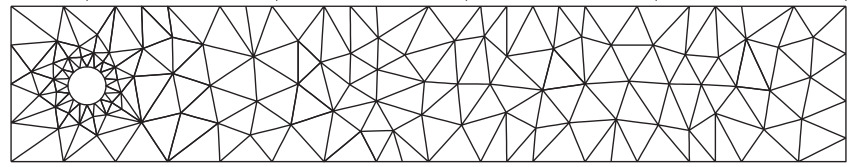
\includegraphics[width=8cm]{images/compgeo/hole}

You can build it 
by hand, or you can use an external mesher library.
Vary the heat conduction coefficient to show the effect of diffusion on the obtained
steady state temperature field.  

%---------------------------------------
\subsection{Diffusion of topography ****}

In a 2D plane assign each node an initial topography $h(x,y,t=0)$ given by 
\[
h(x,y,t=0)= h_0 \sin(\pi x/L_x) + \xi(x,y) \delta h
\]
where $L_x$ and $L_y$ are the dimensions of the domain, $h_0$ is the 
height of the orogen, $xi(x,y)$ is a random perturbation in $[-1,1]$
and $\delta h$ is the amplitude of the perturbation.

We wish to 'erode' the topography by means of a (nonlinear) diffusion law
as in section 2.1.1 of Burov \& Cloetingh \cite{bucl97}.

\begin{enumerate}
\item What are the physical parameters needed to carry out this experiment? 
What are the appropriate boundary conditions? 
What is the steady state? What are the relevant time scales? How should we choose the time step?
\item Write a code which solves the linear diffusion equation until steady state is reached.
Explore the effect of $\delta h$. Compute the slope $\vec\nabla h$ inside each element and plot 
its time evolution. 
\item Implement the nonlinear diffusion law and run the model once again. 
\item If a source term is added to the diffusion equation it is in fact a vertical velocity
($\partial h/\partial t$ has the dimensions of a velocity). Add a source term which generates 
uplift in a symmetric and asymmetric manner.  
\end{enumerate}

\Literature  \cite{thsh14} \cite{ster20}, also check Appendix H. 

%-----------------------------------------------
\subsection{An example of a hand-built triangular mesh}

We start from a 8x5 domain which is tesselated as follows:

\begin{center}
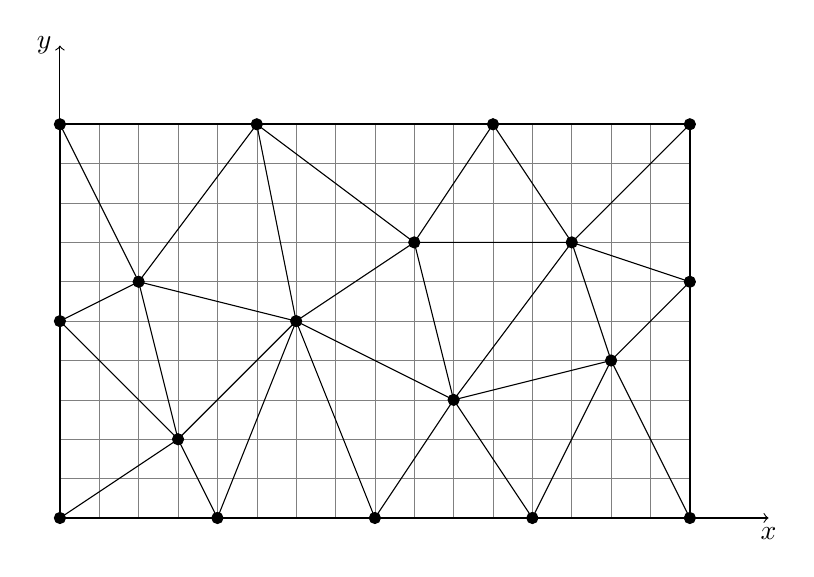
\begin{tikzpicture}
%\draw[fill=gray!8,gray!8](0,0) rectangle (10,7);
\draw[step=0.5cm,gray,very thin] (1,1) grid (9,6); %background grid
\draw[thick] (1,1) -- (9,1) -- (9,6) -- (1,6) -- cycle;  

\draw[thin,->] (1,1) -- (10,1) ; %horizontal axis
\draw[thin,->] (1,1) -- (1,7) ; %horizontal axis
\node[] at (10,0.8){$x$};
\node[] at (0.8,7){$y$};

\draw[] (1,1) -- (2.5,2) -- (4,3.5) -- (5.5,4.5) -- (6.5,6);  %1 6 11 13 14
\draw[] (3,1) -- (4,3.5) -- (6,2.5) -- (7.5,4.5) -- (9,6) ;  %2 11 12 15 16
\draw[] (3,1) -- (2.5,2) -- (1,3.5) -- (2,4) -- (1,6) ;  %2 6 7 8 9
\draw[] (5,1) -- (6,2.5) -- (7,1) -- (8,3) -- (9,4) -- (7.5,4.5) -- (6.5,6) ;  %3 12 4 18 17 15 14
\draw[] (3.5,6) -- (2,4) -- (4,3.5) -- (5,1) ;  %10 8 11 3
\draw[] (2.5,2) -- (2,4) ; %6 8
\draw[] (4,3.5) -- (3.5,6) -- (5.5,4.5) -- (7.5,4.5) ;  %11 10 13 15
\draw[] (9,1) -- (8,3) -- (6,2.5) -- (5.5,4.5) ;  %5 18 12 13
\draw[] (7.5,4.5) -- (8,3) ; %15 18

\draw[black,fill=black] (1,1)     circle (2pt); 
\draw[black,fill=black] (3,1)     circle (2pt); 
\draw[black,fill=black] (5,1)     circle (2pt); 
\draw[black,fill=black] (7,1)     circle (2pt); 
\draw[black,fill=black] (9,1)     circle (2pt); 
\draw[black,fill=black] (2.5,2)   circle (2pt); 
\draw[black,fill=black] (1,3.5)   circle (2pt); 
\draw[black,fill=black] (2,4)     circle (2pt); 
\draw[black,fill=black] (1,6)     circle (2pt); 
\draw[black,fill=black] (3.5,6)   circle (2pt); 
\draw[black,fill=black] (4,3.5)   circle (2pt); 
\draw[black,fill=black] (6,2.5)   circle (2pt); 
\draw[black,fill=black] (5.5,4.5) circle (2pt); 
\draw[black,fill=black] (6.5,6)   circle (2pt); 
\draw[black,fill=black] (7.5,4.5) circle (2pt); 
\draw[black,fill=black] (9,6)     circle (2pt); 
\draw[black,fill=black] (9,4)     circle (2pt); 
\draw[black,fill=black] (8,3)     circle (2pt); 

\end{tikzpicture}\\
\end{center}
         
We can first label the nodes:

\begin{center}
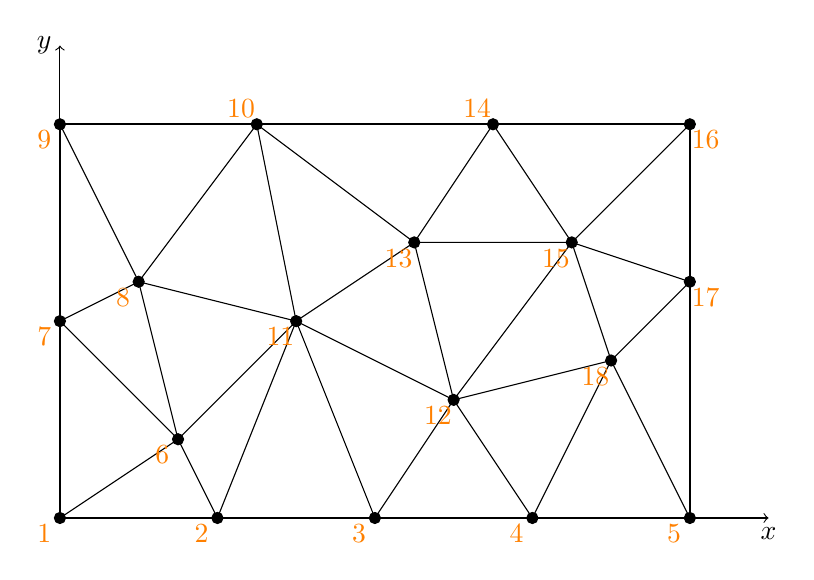
\begin{tikzpicture}
%\draw[fill=gray!5,gray!5](0,0) rectangle (10,7);
%\draw[step=0.5cm,gray,very thin] (1,1) grid (9,6); %background grid
\draw[thick] (1,1) -- (9,1) -- (9,6) -- (1,6) -- cycle;  

\draw[thin,->] (1,1) -- (10,1) ; %horizontal axis
\draw[thin,->] (1,1) -- (1,7) ; %horizontal axis
\node[] at (10,0.8){$x$};
\node[] at (0.8,7){$y$};


\draw[] (1,1) -- (2.5,2) -- (4,3.5) -- (5.5,4.5) -- (6.5,6);  %1 6 11 13 14
\draw[] (3,1) -- (4,3.5) -- (6,2.5) -- (7.5,4.5) -- (9,6) ;  %2 11 12 15 16
\draw[] (3,1) -- (2.5,2) -- (1,3.5) -- (2,4) -- (1,6) ;  %2 6 7 8 9
\draw[] (5,1) -- (6,2.5) -- (7,1) -- (8,3) -- (9,4) -- (7.5,4.5) -- (6.5,6) ;  %3 12 4 18 17 15 14
\draw[] (3.5,6) -- (2,4) -- (4,3.5) -- (5,1) ;  %10 8 11 3
\draw[] (2.5,2) -- (2,4) ; %6 8
\draw[] (4,3.5) -- (3.5,6) -- (5.5,4.5) -- (7.5,4.5) ;  %11 10 13 15
\draw[] (9,1) -- (8,3) -- (6,2.5) -- (5.5,4.5) ;  %5 18 12 13
\draw[] (7.5,4.5) -- (8,3) ; %15 18

\draw[black,fill=black] (1,1)     circle (2pt); \node[] at (0.8,0.8){\color{orange} 1}; %1
\draw[black,fill=black] (3,1)     circle (2pt); \node[] at (2.8,0.8){\color{orange} 2}; %2
\draw[black,fill=black] (5,1)     circle (2pt); \node[] at (4.8,0.8){\color{orange} 3}; %3
\draw[black,fill=black] (7,1)     circle (2pt); \node[] at (6.8,0.8){\color{orange} 4}; %4
\draw[black,fill=black] (9,1)     circle (2pt); \node[] at (8.8,0.8){\color{orange} 5}; %5
\draw[black,fill=black] (2.5,2)   circle (2pt); \node[] at (2.3,1.8){\color{orange} 6}; %6
\draw[black,fill=black] (1,3.5)   circle (2pt); \node[] at (0.8,3.3){\color{orange} 7}; %7
\draw[black,fill=black] (2,4)     circle (2pt); \node[] at (1.8,3.8){\color{orange} 8}; %8
\draw[black,fill=black] (1,6)     circle (2pt); \node[] at (0.8,5.8){\color{orange} 9}; %9
\draw[black,fill=black] (3.5,6)   circle (2pt); \node[] at (3.3,6.2){\color{orange} 10};%10
\draw[black,fill=black] (4,3.5)   circle (2pt); \node[] at (3.8,3.3){\color{orange} 11};%11
\draw[black,fill=black] (6,2.5)   circle (2pt); \node[] at (5.8,2.3){\color{orange} 12};%12
\draw[black,fill=black] (5.5,4.5) circle (2pt); \node[] at (5.3,4.3){\color{orange} 13};%13
\draw[black,fill=black] (6.5,6)   circle (2pt); \node[] at (6.3,6.2){\color{orange} 14};%14
\draw[black,fill=black] (7.5,4.5) circle (2pt); \node[] at (7.3,4.3){\color{orange} 15};%15
\draw[black,fill=black] (9,6)     circle (2pt); \node[] at (9.2,5.8){\color{orange} 16};%16
\draw[black,fill=black] (9,4)     circle (2pt); \node[] at (9.2,3.8){\color{orange} 17};%17
\draw[black,fill=black] (8,3)     circle (2pt); \node[] at (7.8,2.8){\color{orange} 18};%18
\end{tikzpicture}\\
\end{center}

and then label the elements:

\begin{center}
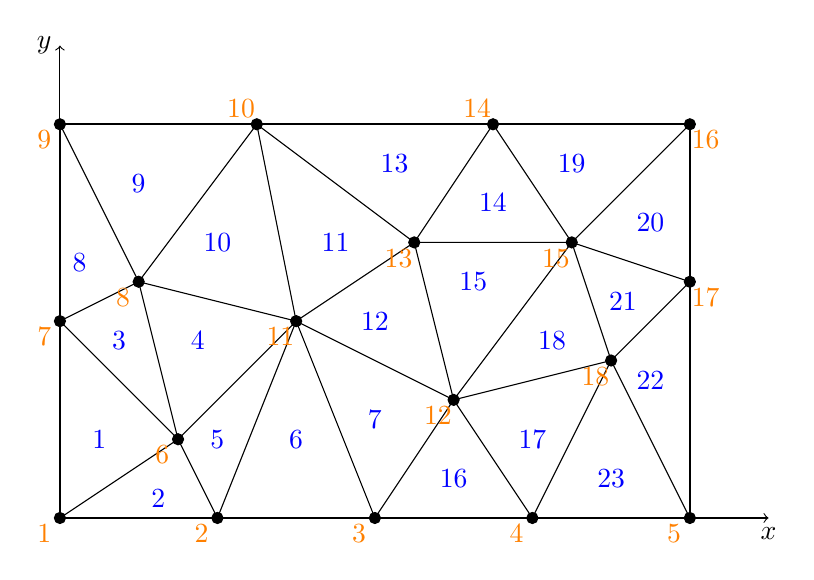
\begin{tikzpicture}
%\draw[fill=gray!5,gray!5](0,0) rectangle (10,7);
%\draw[step=0.5cm,gray,very thin] (1,1) grid (9,6); %background grid
\draw[thick] (1,1) -- (9,1) -- (9,6) -- (1,6) -- cycle;  

\draw[thin,->] (1,1) -- (10,1) ; %horizontal axis
\draw[thin,->] (1,1) -- (1,7) ; %horizontal axis
\node[] at (10,0.8){$x$};
\node[] at (0.8,7){$y$};


\draw[] (1,1) -- (2.5,2) -- (4,3.5) -- (5.5,4.5) -- (6.5,6);  %1 6 11 13 14
\draw[] (3,1) -- (4,3.5) -- (6,2.5) -- (7.5,4.5) -- (9,6) ;  %2 11 12 15 16
\draw[] (3,1) -- (2.5,2) -- (1,3.5) -- (2,4) -- (1,6) ;  %2 6 7 8 9
\draw[] (5,1) -- (6,2.5) -- (7,1) -- (8,3) -- (9,4) -- (7.5,4.5) -- (6.5,6) ;  %3 12 4 18 17 15 14
\draw[] (3.5,6) -- (2,4) -- (4,3.5) -- (5,1) ;  %10 8 11 3
\draw[] (2.5,2) -- (2,4) ; %6 8
\draw[] (4,3.5) -- (3.5,6) -- (5.5,4.5) -- (7.5,4.5) ;  %11 10 13 15
\draw[] (9,1) -- (8,3) -- (6,2.5) -- (5.5,4.5) ;  %5 18 12 13
\draw[] (7.5,4.5) -- (8,3) ; %15 18

\draw[black,fill=black] (1,1)     circle (2pt); \node[] at (0.8,0.8){\color{orange} 1}; %1
\draw[black,fill=black] (3,1)     circle (2pt); \node[] at (2.8,0.8){\color{orange} 2}; %2
\draw[black,fill=black] (5,1)     circle (2pt); \node[] at (4.8,0.8){\color{orange} 3}; %3
\draw[black,fill=black] (7,1)     circle (2pt); \node[] at (6.8,0.8){\color{orange} 4}; %4
\draw[black,fill=black] (9,1)     circle (2pt); \node[] at (8.8,0.8){\color{orange} 5}; %5
\draw[black,fill=black] (2.5,2)   circle (2pt); \node[] at (2.3,1.8){\color{orange} 6}; %6
\draw[black,fill=black] (1,3.5)   circle (2pt); \node[] at (0.8,3.3){\color{orange} 7}; %7
\draw[black,fill=black] (2,4)     circle (2pt); \node[] at (1.8,3.8){\color{orange} 8}; %8
\draw[black,fill=black] (1,6)     circle (2pt); \node[] at (0.8,5.8){\color{orange} 9}; %9
\draw[black,fill=black] (3.5,6)   circle (2pt); \node[] at (3.3,6.2){\color{orange} 10};%10
\draw[black,fill=black] (4,3.5)   circle (2pt); \node[] at (3.8,3.3){\color{orange} 11};%11
\draw[black,fill=black] (6,2.5)   circle (2pt); \node[] at (5.8,2.3){\color{orange} 12};%12
\draw[black,fill=black] (5.5,4.5) circle (2pt); \node[] at (5.3,4.3){\color{orange} 13};%13
\draw[black,fill=black] (6.5,6)   circle (2pt); \node[] at (6.3,6.2){\color{orange} 14};%14
\draw[black,fill=black] (7.5,4.5) circle (2pt); \node[] at (7.3,4.3){\color{orange} 15};%15
\draw[black,fill=black] (9,6)     circle (2pt); \node[] at (9.2,5.8){\color{orange} 16};%16
\draw[black,fill=black] (9,4)     circle (2pt); \node[] at (9.2,3.8){\color{orange} 17};%17
\draw[black,fill=black] (8,3)     circle (2pt); \node[] at (7.8,2.8){\color{orange} 18};%18


\node[] at (1.5,2) {\color{blue}1};
\node[] at (2.25,1.25) {\color{blue}2};
\node[] at (1.75,3.25) {\color{blue}3};
\node[] at (2.75,3.25) {\color{blue}4};
\node[] at (3,2) {\color{blue}5};
\node[] at (4,2) {\color{blue}6};
\node[] at (5,2.25) {\color{blue}7};
\node[] at (1.25,4.25) {\color{blue}8};
\node[] at (2,5.25) {\color{blue}9};
\node[] at (3,4.5) {\color{blue}10};
\node[] at (4.5,4.5) {\color{blue}11};
\node[] at (5,3.5) {\color{blue}12};
\node[] at (5.25,5.5) {\color{blue}13};
\node[] at (6.5,5) {\color{blue}14};
\node[] at (6.25,4) {\color{blue}15};
\node[] at (6,1.5) {\color{blue}16};
\node[] at (7,2) {\color{blue}17};
\node[] at (7.25,3.25) {\color{blue}18};
\node[] at (7.5,5.5) {\color{blue}19};
\node[] at (8.5,4.75) {\color{blue}20};
\node[] at (8.15,3.75) {\color{blue}21};
\node[] at (8.5,2.75) {\color{blue}22};
\node[] at (8,1.5) {\color{blue}23};


\end{tikzpicture}\\
\end{center}

We can finally build the connectivity array by hand:

\noindent
icon(1,{\color{blue}1})={\color{orange}1}\\
icon(2,{\color{blue}1})={\color{orange}6}\\
icon(3,{\color{blue}1})={\color{orange}7}\\
icon(1,{\color{blue}2})={\color{orange}1}\\
icon(2,{\color{blue}2})={\color{orange}2}\\
icon(3,{\color{blue}2})={\color{orange}6}\\
icon(1,{\color{blue}3})={\color{orange}7}\\
icon(2,{\color{blue}3})={\color{orange}6}\\
icon(3,{\color{blue}3})={\color{orange}8}\\
...\\
icon(1,{\color{blue}12})={\color{orange}11}\\
icon(2,{\color{blue}12})={\color{orange}12}\\
icon(3,{\color{blue}12})={\color{orange}13}\\
...\\
icon(1,{\color{blue}19})={\color{orange}14}\\
icon(2,{\color{blue}19})={\color{orange}15}\\
icon(3,{\color{blue}19})={\color{orange}16}\\


The labelling of nodes and elements above is done by a human so it starts at 1. When 
implementing this in python, you know what to do ...
